\end{multicols}
\newpage
\section{Studienplan(ung) für jeden}
\begin{multicols}{2}
% uiuiu, hier muss ja alles neu strukturiert werden

%	Freiheit und Verantwortung
%	Ordnungen
%	Studienplanung grob
%	Module und Co.
%	Welche Fächer gibt es
%	Der allgemeine Stundenplan
%	Niveau ist keine Hautcreme
%	Interview mit Prof. Struckmann
%	Bachelor und Master im Vergleich
%		Herden und Rudel
%		Stunden- und Studienpläne

\subsection{Sonstige Informationen}
%TODO raus damit

\subsection{Hinweise zu Lehrveranstaltungen}

Du wirst sehr bald feststellen, dass es verschiedene Lerntypen gibt. Manche
deiner Kommilitonen werden kaum eine Vorlesung besuchen, sondern stattdessen die großen
und kleinen Übungen verschlingen. Wieder andere lassen sich sowieso kaum im
Hörsaal blicken, sondern können am besten zu Hause oder in der Uni-Bibliothek
autodidaktisch lernen.

Wenn trotz Vorlesungen, großer und kleiner Übungen noch Fragen
auftreten, hilft dir das Gespräch mit HiWis oder Kommilitonen und der Blick in
entsprechende Literatur.
Wichtig: Kaufe nicht gleich jedes empfohlene Buch neu,
das ist Geldverschwendung. Frage höhere Semester nach wirklich sinnvoller
Literatur, leihe dir die Bücher aus der UB, gebrauchte Bücher gibt es
günstig z.B. in der Newsgroup \url{http://groups.google.de/group/braunschweig.kaufrausch/} (siehe den Artikel
ab Seite \pageref{elekinf}). 

An der Uni wirst du nicht wie in der
Schule oder der betrieblichen Ausbildung umsorgt, du trägst ein wesentlich höheres
Maß an Eigenverantwortung. Zur Orientierung in der ersten Zeit ist ein
Ansprechpartner unentbehrlich. Wenn die Kommilitonen aus
deinem eigenen Semester nicht weiterhelfen können, dann vielleicht dein/e TutorIn oder andere
Studierende im höheren Semester (zum Beispiel Mitbewohner, Fachgruppe).


\subsection{Die Prüfungsordnung}
\label{po}
	An einer Universität gibt es tausende Regeln und Ordnungen. Die wichtigste ist die Prüfungsordnung: Sie enthält Antworten auf 95\% aller Fragen, die im Studium auftreten - nicht nur, wenn es um die eigentlichen Prüfungen geht. Die genaue Bezeichnung lautet \emph{Besonderer Teil der Prüfungsordnung für den (Bachelor-/Master-)studiengang Informatik der Technischen Universität Braunschweig}. Und da sie weder besonders lang, noch kompliziert geschrieben ist, sollte sie jeder Student mindestens einmal lesen.

	Dann gibt es noch die APO, die Allgemeine Prüfungsordnung. Sie gilt uniweit für alle Studiengänge, doch die beiden BPOs überschreiben die meisten APO-Regelungen.

	Wenn du es noch nicht getan hast, lade dir deine aktuelle Prüfungsordnung am besten von \url{http://www.tu-braunschweig.de/fk1/service/informatik/dokumente} herunter. 




% !TEX root = ../../1-te.tex

\subsection{Studienplan}
	\label{bach_studienplan}
	\tocheck{5}{Stimmt die Anzahl Pflichtveranstaltungen noch? Mit aktuellem Stundenplan abgleichen!}
	Wie du wahrscheinlich bereits in deinem Stundenplan festgestellt hast, musst du im ersten Semester \iftoggle{winter}{vier}{vier} Pflichtveranstaltungen hören. Doch die Bezeichnung Pflichtverantstaltung sagt bloß aus, dass du die Veranstaltung \emph{irgendwann} einmal hören musst, um deinen Bachelor abzuschließen. Die zeitliche Abfolge der Veranstaltungen darfst du aber selbst festlegen. Der Fakultäts-Musterstudienplan bietet hier eine gute Orientierungsmöglichkeit. Du musst dich aber nicht daran halten. Niemand zwingt dich eine Veranstaltung zu hören oder hält dich davon ab. Du kannst dich eigentlich in jede Vorlesung setzen, auch ohne hinterher an der Prüfung teilnehmen zu müssen -- allerdings gibt es dann auch keine Punkte dafür. Hier bieten sich zum Beispiel Module aus dem Wahlplichtbereich Informatik an, die eventuell nur alle 2 Jahre angeboten werden und über mehrere Semester gehen. Bei den (Pflicht-)Modulen der Informatik musst du jedoch beachten, dass einige Module auf anderen aufbauen. Zum Beispiel sollten Programmiergrundlagen in den ersten zwei Semestern erarbeitet werden und mit Theoretische Informatik II wirst du dich schwer tun, wenn du TheoInf I nicht gehört hast.

	Damit sich dein Studium nicht unnötig verlängert, solltest du darauf achten, in jedem Semester rund 30 Leistungspunkte zu erwerben.


\label{musterstudienplan}
\begin{figure}[h]
  \centering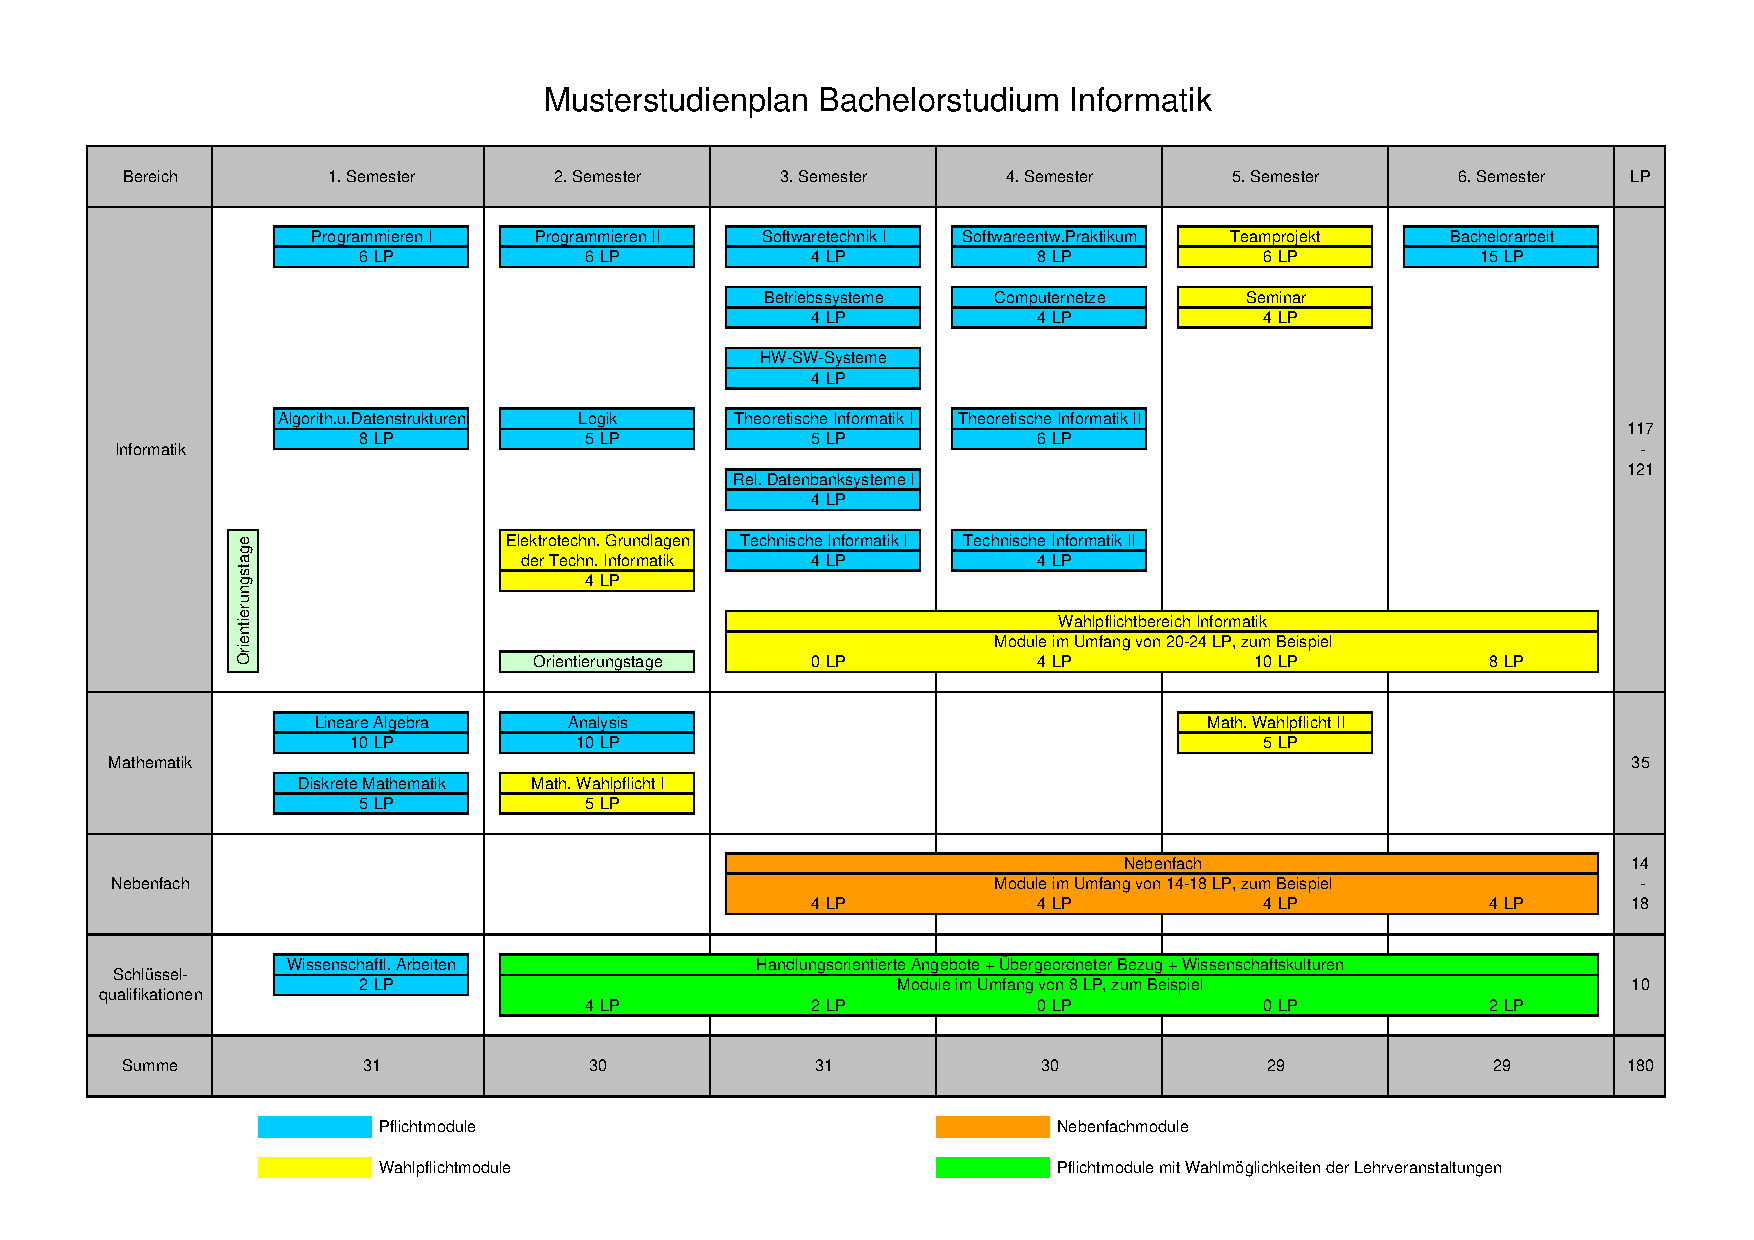
\includegraphics[angle=90,totalheight=\textheight, width=\textwidth ]{texte/bachelor/studienplan.pdf}
\end{figure}

\label{studienplan_neu}
\begin{figure}[h]
  \centering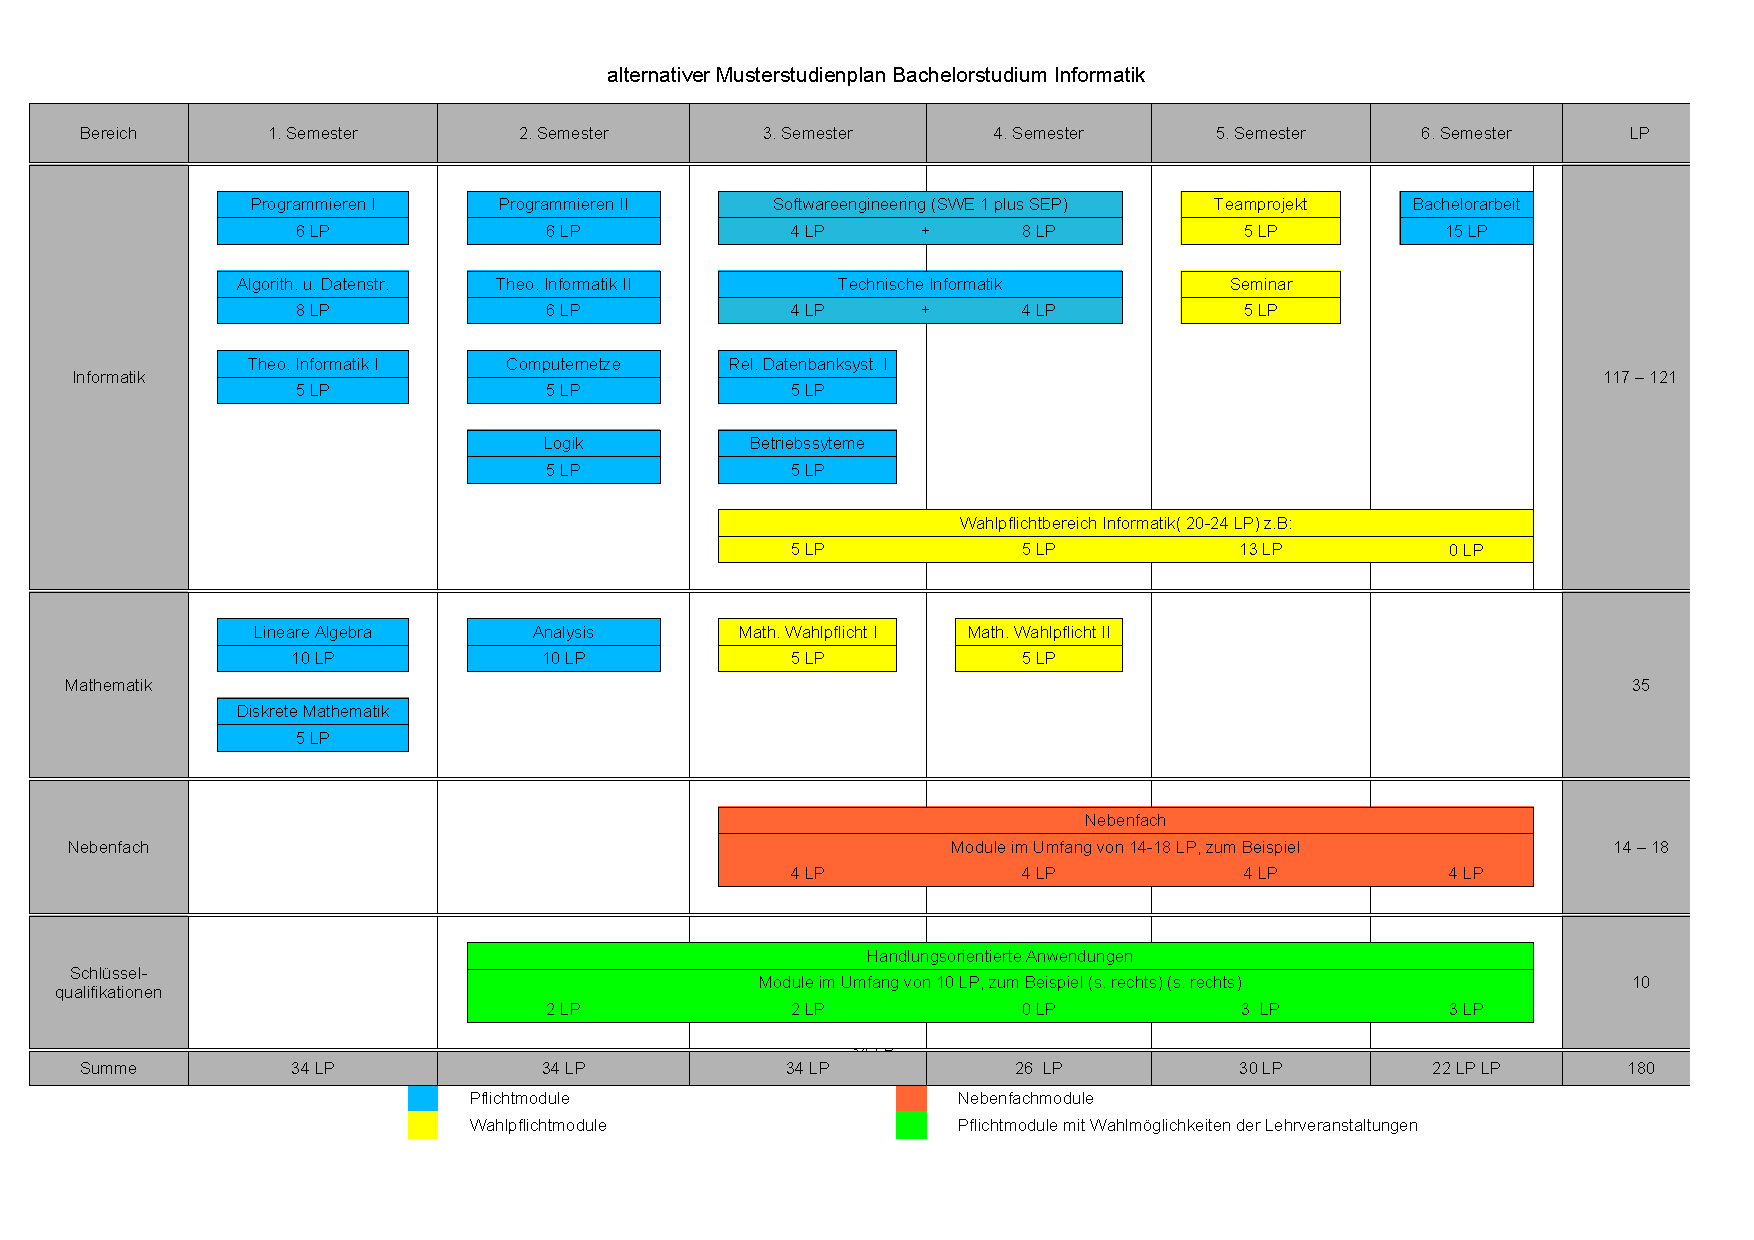
\includegraphics[angle=90,totalheight=\textheight, width=\textwidth ]{texte/bachelor/studienplan_neu.pdf}
\end{figure}


\subsection{Stunden- und Semesterplan}
 
Im Vergleich zum Bachelorstudium an der TU-BS bietet der Master
verblüffende Freiheiten in der Fächerwahl. Auch wer die Redewendung
bisher dumm fand, lernt spätestens hier was "`die Qual der Wahl"'
bedeutet. Daher sind dieses und die folgenden Unterkapitel auch in erster
Linie für Masterstudenten gedacht. Allerdings werden mit einigen
Themen auch Bachelorstudenten in Berührung kommen, aber erst ab den
3. Semester. Bei Unterschieden zwischen den Studiengängen gehen wir
kurz darauf ein.\\\\
Zu Beginn jedes Semesters muss man sich selbständig entscheiden, welche Fächer man belegen möchte (und kann) und sich danach den Stundenplan zusammenstellen. Im Gegensatz zu den alteingessenen Bacheloranden aus Braunschweig steht man recht unvorbereitet vor einer ganz und gar nicht trivialen Aufgabe, die man am besten noch vor dem ersten Studientag erledigen sollte. Vielleicht hatte dein Bachelor kaum Wahlmöglichkeiten und das Zusammenstellen eines eigenen Stundenplans ist für dich ungewohnt. Und selbst wenn du diese Freiheiten schon im Bachelor hattest, so sind die Rahmenbedinungen und Feinheiten hier sicherlich ganz andere.

Und anders als im Bachelor, bei dem die meisten Vorlesungen erst in der zweiten Woche beginnen, starten viele Mastervorlesungen schon in der ersten Woche, schlimmstenfall schon Montag früh. Die erste Vorlesung zu verpassen ist nun auch nicht so schlimm, aber wenn mans vermeiden kann\ldots Es ist übrigens auch nicht ganz leicht, den Vorlesungsstart eines Faches herauszufinden, somit wirst du in der ersten (und evtl. auch zweiten) Woche oft vor verschlossenen Türen oder leeren Räumen stehen.







\subsection{Studienplan und Reihenfolge}
Mindestens so frei wie die Wahl der Fächer ist auch die Wahl der Reihenfolge, in der man diese belegt. Es kursieren Studienpläne für den Master, die vorschlagen, bestimmte Module im ersten Semester zu machen (z.B. das Seminar), und andere im zweiten und dritten, etc. All dies sind höchstens gut gemeinte Tipps, letzlich muss ja nichtmals die Masterarbeit unbedingt am Ende stehen, und zur Idee, das Seminar im ersten Semester zu belegen, siehe auch den nächsten Absatz\ldots
          



